\documentclass{ijitcs}

\usepackage{amsmath,amssymb,amsfonts,multirow,array}
\usepackage{algorithmic}
\usepackage{algorithm}
\usepackage{textcomp}
\usepackage{xcolor}
\usepackage{booktabs}
\usepackage{hyperref}
\usepackage{tikz}
\usetikzlibrary{arrows.meta,positioning,shapes.geometric,patterns,decorations.pathreplacing}

% --- Highlighting policy (Requirement 9) ---
% Previous review-round revisions are now the accepted baseline: rendered in normal (black).
\newcommand{\rev}[1]{#1}
% This camera-ready resubmission round's changes are highlighted in a single color (red).
% Note: \cr is a TeX alignment primitive, so this macro is named \crx to avoid a clash.
\newcommand{\crx}[1]{{\color{red}#1}}

% --- Declarations block (journal template style: titled sub-blocks) ---
\newenvironment{AllDeclarations}{}{}
\newcommand{\declitem}[2]{\par\medskip\noindent{\bfseries #1}\par\nobreak\vspace{1pt}\noindent #2\par}

\IjitcsSet{
    title = {Physics-Aware Rule-Based Temporal Filtering for Scalable Vehicle Re-Identification},
    volume = {},
    issue = {},
    year = {},
    month = {},
    startpage = {},
    endpage = {},
    doi = {},
    abstract = {
        \rev{Vehicle re-identification (Re-ID) must often search very large galleries even when most candidates are physically implausible. We introduce a physics-aware rule-based temporal consistency module (TCM) as an efficiency-first temporal prior rather than a replacement for the visual backbone. The module models the camera network as a weighted graph, estimates driving distance with the Haversine formula and a global tortuosity scalar of 1.4 in the current VeRi-776 study, assigns road-type speed profiles, and expands the upper travel bound during rush hour. In targeted camera-to-camera tracking the TCM can hard-gate impossible transfers; in full-gallery retrieval it applies a soft penalty instead of irrevocable deletion, which reduces brittleness under route uncertainty or timestamp drift. On VeRi-776, the TCM reduces the candidate set by 338$\times$ in sequential tracking, pruning 99.70\% of comparisons before visual ranking. The effect on retrieval accuracy is modest---mean average precision rises from 82.1\% to 82.5\% while rank-1 accuracy remains essentially unchanged---so we position the method primarily as a zero-training efficiency layer. Metadata-sensitivity checks under a 30\,s clock guard band, independent 50\,m camera-coordinate perturbations, and a 20\% higher upper-speed bound show only minor changes in temporal retention. Metropolitan-scale results are therefore reported as throughput projections, while validation on larger benchmarks such as VeRi-Wild and CityFlow remains future work.}
    },
    keywords = {Vehicle Re-Identification, Temporal Consistency, Spatio-Temporal Constraints, Camera Network Modeling, Real-Time Tracking, Intelligent Transportation Systems},
    received = {\crx{14 March, 2026; Revised: 07 May, 2026; Accepted: 09 July, 2026; Published: XX Month, 2026}}
}

\author*{Chris Thomas Saji}{\crx{Department of Artificial Intelligence and Data Science}, Rajagiri School of Engineering \& Technology (Autonomous), Kochi, India}{chris.saji001@gmail.com}{https://orcid.org/0009-0005-4425-0540}

\author{Jithin Mathews}{\crx{Department of Artificial Intelligence and Data Science}, Rajagiri School of Engineering \& Technology (Autonomous), Kochi, India}{jithinm@rajagiritech.edu.in}{https://orcid.org/0000-0001-6279-7279}


\thispagestyle{thefirstpage}
\begin{document}


\maketitle


\section{Introduction}
Vehicle re-identification (Re-ID) deals with a deceptively simple question: given a snapshot of a car from one camera, can we find that exact car in footage from a completely different camera? The task matters for traffic analysis, stolen-vehicle recovery, forensic investigations, and toll enforcement. License plate recognition (LPR) can sometimes do this, but plates get obscured by dirt, blur, bad angles, and even intentional tampering, so appearance-based Re-ID has emerged as a complementary and sometimes necessary alternative.

Scale is the first headache. A mid-sized city might run a few thousand cameras that collectively record millions of vehicle sightings per day. A brute-force system would compare every query against every gallery image---an $O(N)$ sweep through high-dimensional feature space that quickly becomes too slow for anything resembling real time.

The second headache is visual ambiguity, and it is worse for vehicles than for people. Two white Toyota Corollas from the same model year are, for practical purposes, pixel-identical from the rear. Meanwhile, a single vehicle can look entirely different when shot from the front versus the side, or in midday sun versus under a streetlight at night. The literature calls these problems \textit{inter-class similarity} and \textit{intra-class variance}, respectively. Together, they put a hard ceiling on what appearance alone can do---especially in cities full of fleet taxis, delivery vans, and rental cars that share the same paint job.

Modern methods lean on CNNs [1] or Vision Transformers [2,3] to pull out fine-grained cues like bumper stickers, scratches, and aftermarket accessories. These features work well, but they treat every image as if it exists in a vacuum. They ignore an obvious physical fact: a car seen at Camera~A at time $t_1$ simply cannot show up at Camera~B, five kilometers away, one second later. It has to obey speed limits, traffic lights, and the geometry of the road network.

Some recent work [4,5] tries to fold spatio-temporal information into the pipeline through learned transition models, including LSTMs and graph networks. We see three recurring problems. These models are black boxes---uncomfortable when the output feeds into law-enforcement decisions. They need large annotated datasets with precise, synchronized timestamps across every camera pair, and assembling that kind of training set is expensive. And perhaps most importantly, a learned model finds statistical correlations, not physical laws, so it might assign a small-but-nonzero probability to a transition that is flatly impossible. A rule-based check would give it exactly zero.

Our response is a \textbf{Rule-Based Temporal Consistency Module (TCM)}. The idea is simple: model the camera network as a graph whose edges carry driving distances and speed profiles, then \rev{either reject or softly down-weight} any query--gallery pair whose time gap violates the resulting travel-time bounds. No neural network, no training data, no GPUs for the filter itself. We plug TCM in \textit{before} the visual ranker, so it never touches the appearance features, meaning it \rev{interfaces cleanly with any backbone even though the present paper validates the gain only with TransReID}.

\rev{The revised manuscript intentionally treats efficiency as the hero metric. The +0.4\,pp mAP change is reported as a secondary effect of pruning long-tail false positives, not as evidence that the temporal module resolves the hardest top-rank visual ambiguities by itself; the visual backbone remains the dominant Rank-1 bottleneck.}

We make four contributions:
\begin{enumerate}
    \item \rev{A graph-based temporal prior that makes the tortuosity assumption explicit: the current study uses a single global scalar $\tau = 1.4$, while the formulation also admits edge-specific coefficients from map services such as OpenStreetMap.}
    \item \rev{A dual-mode filtering policy: a hard gate for targeted camera-to-camera tracking and a soft additive penalty for full-gallery retrieval, augmented with a deployment guard band for timestamp jitter.}
    \item \rev{Experiments on VeRi-776 showing a \textbf{338$\times$ speedup} (99.70\% search-space reduction) in sequential tracking while leaving retrieval accuracy essentially unchanged, which positions TCM as an efficiency layer rather than a new visual discriminant.}
    \item \rev{A robustness analysis covering clock guard bands, camera-coordinate perturbations, upper-speed tolerance for speeders, offline-versus-online complexity, and the remaining limitations around dwell time, larger datasets, and multi-backbone validation.}
\end{enumerate}


\loadmaingeometry

\section{Related Work}

\subsection{Deep Learning for Visual Feature Extraction}
Before deep learning took over, Re-ID systems cobbled together handcrafted descriptors---SIFT, HOG, color histograms---and the results were mediocre, rarely cracking 30\% mAP on hard benchmarks. Ye et al.\ [6] survey the shift in detail: deep learning replaced nearly every component of the re-identification pipeline, and vehicle Re-ID followed the same trajectory.

He et al.\ [1] introduced residual connections that made it practical to train networks with 100+ layers. ResNet-50 quickly became the default backbone for Re-ID: deep enough to capture both coarse shape and fine texture, yet trainable without vanishing gradients. On the training side, Luo et al.\ [7] showed that a collection of simple tricks---warm-up learning rate, BNNeck, label smoothing, and random erasing augmentation---can push a plain ResNet-50 baseline surprisingly close to state-of-the-art without any architectural novelty. Their ``bag of tricks'' paper has become the de facto recipe for training Re-ID models and influenced most subsequent work, including ours.

Vision Transformers (surveyed by Khan et al.\ [3]) shook things up further. Dosovitskiy et al.\ [2] showed that slicing an image into patches and running a Transformer over them can match or beat CNNs on standard benchmarks. The payoff for Re-ID is global self-attention: a single layer can relate a roof rack to a bumper sticker on the opposite end of the car, which is exactly what you want when parts of the vehicle are blocked.

\subsection{Appearance-Based Vehicle Re-ID}
Metric learning for vehicle Re-ID dates back at least to Liu et al.\ [8], whose Deep Relative Distance Learning (DRDL) system trained a network to pull embeddings of the same vehicle closer while pushing apart those of different vehicles. DRDL worked, but it operated on whole-image features and fell short when the distinguishing mark was small---a scratch on the fender, a particular sticker. \rev{Liu et al. later extended this line with a progressive vehicle re-identification formulation for urban surveillance [9] and then with the multimodal PROVID framework [10], both of which are also standard citations associated with the VeRi benchmark family.} On a different track, Li et al.\ [11] adapted CLIP for Re-ID by learning modality-specific prompts and got strong numbers on both person and vehicle benchmarks, hinting that cross-modal pre-training may eventually rival metric learning in importance.

Zhou and Shao [12] attacked viewpoint variation head-on, learning angle-specific feature representations and fusing them through attention so that a front-view query can match a rear-view gallery image of the same car. Their key point: viewpoint is not noise but a structured variable worth modeling on its own. Chen et al.\ [13] pushed the idea further into the temporal domain with spatial-temporal graph neural networks that jointly model appearance and inter-camera transition patterns. Their formulation captures both local visual cues and network-level constraints---goals we share, though we enforce temporal consistency through physics rather than learned graph weights.

The scale of the problem keeps growing too. The 7th AI City Challenge (Naphade et al.\ [14]) ran vehicle tracking and Re-ID tracks across hundreds of real urban cameras. One pattern stands out across multiple challenge editions: winning systems almost always pair a strong visual backbone with some form of explicit spatio-temporal reasoning. Our TCM takes that lesson to its logical extreme.

On the data side, Zheng et al.\ [15] pooled several vehicle Re-ID datasets into VehicleNet and pre-trained on the combined set. Representations trained this way transferred better to held-out domains---a reminder that data scale matters at least as much as architecture. Lou et al.\ [16] released VERI-Wild, a large-scale dataset spanning 174 cameras with messy real-world conditions: rain, night, heavy occlusion. Methods tuned on the relatively clean VeRi-776 often fell apart on VERI-Wild, which forced the community to take robustness more seriously.

TransReID [17] brought Transformers into the Re-ID space with two notable design choices: a jigsaw patch module (JPM) that shuffles patches during training so the network cannot rely on spatial layout, and side information embeddings (SIE) that encode which camera captured each image and from what angle. It currently sits at or near the top of most Re-ID leaderboards, and we use it as our visual backbone throughout this paper.

All of these methods share one blind spot: if two genuinely different cars look the same (same make, same color, same year), no visual feature, however sophisticated, can tell them apart. In any city with a taxi fleet or a delivery company, this comes up every day.

\subsection{Spatio-Temporal Approaches for Re-ID}
The idea of using time and location to help Re-ID is not new, but implementations differ sharply in philosophy. Wang et al.\ [4] baked spatial-temporal regularization directly into the training loss, learning a probability distribution over camera-pair transitions at different hours. The accuracy improved, but the temporal model lives inside the network weights. You cannot inspect it, tweak it for a new city, or even explain why a particular match was rejected.

Shen et al.\ [5] proposed generating candidate vehicle trajectories (``paths'') through the camera graph and scoring each path for visual and temporal consistency. Reasoning over full trajectories rather than isolated pairs gives more globally coherent results, but path enumeration blows up combinatorially, and the temporal scoring is still a learned neural module with the usual opacity and data requirements.

The 8th AI City Challenge [18] at CVPR~2024 doubled down on city-scale multi-camera Re-ID and tracking, and the winning entries all used some form of spatio-temporal filtering or graph-based transition model alongside their visual backbones. At this point it is hard to argue that temporal reasoning is optional; appearance-only pipelines seem to have hit diminishing returns.

The key philosophical difference between these methods and ours boils down to \textit{statistics vs.\ physics}. Learned models pick up on correlations---``transitions between cameras 3 and 7 usually take about four minutes.'' Our approach encodes a harder claim: ``a car \textit{cannot} cover 2\,km in under 60 seconds on a residential road with a 40\,km/h limit.'' A learned model might still assign a tiny probability to that impossible event. Our filter assigns exactly zero.

\subsection{Multi-Camera Tracking and Re-ID}
Re-ID and multi-target multi-camera (MTMC) tracking overlap heavily. Ristani and Tomasi [19] found that a well-engineered feature extractor plus simple association heuristics can rival far more complex MTMC systems---a result that encouraged us to keep temporal reasoning separate from feature learning rather than entangling the two. Tang et al.\ [20] introduced CityFlow, a city-scale benchmark with over 200 cameras in real urban traffic. Once camera counts move from the tens to the hundreds, exhaustive pairwise visual comparison stops being practical regardless of backbone quality, and some form of pre-filtering becomes a structural requirement.

\subsection{Camera Network and Traffic Modeling}
Modeling camera networks as graphs is standard practice in multi-target tracking, but most prior work couples the graph with a learned transition model that needs synchronized timestamp labels across every camera pair. We sidestep that requirement entirely by borrowing from traffic engineering instead.

Road tortuosity (the ratio of actual driving distance to straight-line distance) is a well-studied quantity in transportation geography. In typical urban grids the factor falls between 1.2 and 1.6, depending on how regular the street layout is and whether one-way streets or restricted zones force detours. We use this simple multiplier to convert Haversine (great-circle) distances into reasonable driving-distance estimates, no map API needed.

Travel-time variation by time of day is equally well characterized. Morning and evening rush hours can inflate arterial travel times by 30--50\% relative to free-flow conditions. We fold this into our model with a binary expansion factor $\alpha(t)$ that widens the allowed time window during peak periods. The approach is deliberately coarse; finer models are certainly possible, but they would add parameters without changing the core mechanism.


\section{Methodology}

\subsection{System Overview}
The idea behind our system is straightforward: before burning compute on visual comparisons, check whether a candidate match is even physically possible. \rev{Fig.~\ref{fig:system} lays out the pipeline. In targeted sequential tracking, the temporal module acts as a hard gate because the operator is asking a specific camera-to-camera question. In full-gallery retrieval, we use the same feasibility test as a soft prior: implausible candidates are down-weighted rather than deleted. This distinction is important for robustness.} A query observation from Camera $c_q$ at time $t_q$ triggers a physics check on every gallery candidate---could a vehicle realistically travel between these two cameras in the observed time gap? Anything that fails gets tossed, leaving a filtered subset $\mathcal{G}_{valid}$. Only then does the Re-ID backbone (TransReID in our case) rank what remains by visual similarity. The reason the payoff is so large comes down to a cost asymmetry: each TCM check is an $O(1)$ arithmetic operation, while a single feature-space similarity score requires a 768-dimensional dot product.

\begin{figure}[htbp]
\centering
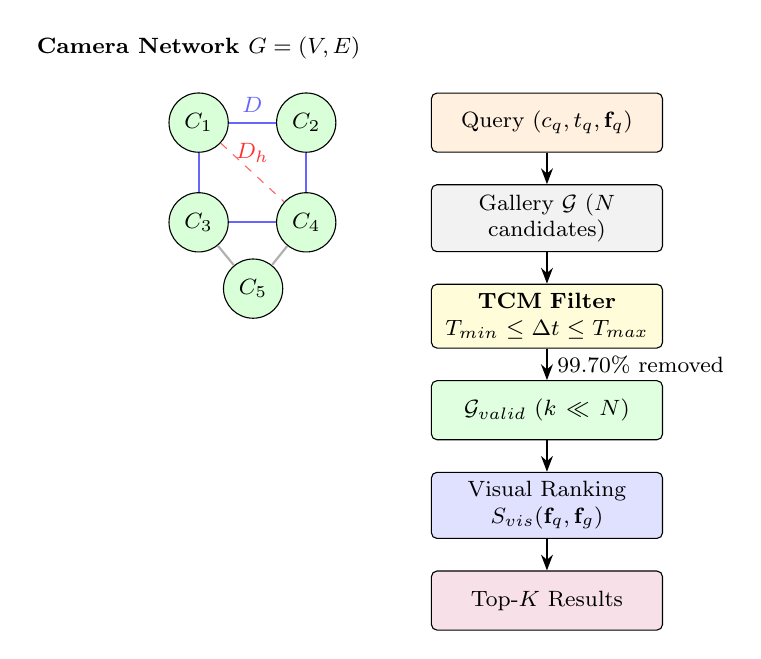
\begin{tikzpicture}[
    node distance=0.6cm and 0.4cm,
    block/.style={rectangle, draw, fill=blue!8, text width=2.7cm, text centered, minimum height=0.75cm, font=\footnotesize, rounded corners=2pt},
    arrow/.style={-{Stealth[length=2mm]}, thick},
    cam/.style={circle, draw, fill=green!15, minimum size=0.55cm, font=\footnotesize\bfseries},
]
% Camera Network (left side)
\node[font=\footnotesize\bfseries] (netlabel) {Camera Network $G=(V,E)$};
\node[cam, below=0.3cm of netlabel] (c1) {$C_1$};
\node[cam, right=0.6cm of c1] (c2) {$C_2$};
\node[cam, below=0.5cm of c1] (c3) {$C_3$};
\node[cam, right=0.6cm of c3] (c4) {$C_4$};
\node[cam, below right=0.3cm and 0.15cm of c3] (c5) {$C_5$};

\draw[thick, blue!60] (c1) -- node[above, font=\footnotesize] {$D$} (c2);
\draw[thick, blue!60] (c1) -- (c3);
\draw[thick, blue!60] (c2) -- (c4);
\draw[thick, blue!60] (c3) -- (c4);
\draw[thick, gray!60] (c3) -- (c5);
\draw[thick, gray!60] (c4) -- (c5);

% Dashed line for haversine
\draw[dashed, red!60, thin] (c1) -- (c4) node[midway, above, font=\footnotesize, red!80] {$D_h$};

% Pipeline (right side)
\node[block, right=1.2cm of c2, fill=orange!12] (query) {Query $(c_q, t_q, \mathbf{f}_q)$};
\node[block, below=0.4cm of query, fill=gray!10] (gallery) {Gallery $\mathcal{G}$ ($N$ candidates)};
\node[block, below=0.4cm of gallery, fill=yellow!15] (tcm) {\textbf{TCM Filter}\\$T_{min} \leq \Delta t \leq T_{max}$};
\node[block, below=0.4cm of tcm, fill=green!12] (filtered) {$\mathcal{G}_{valid}$ ($k \ll N$)};
\node[block, below=0.4cm of filtered, fill=blue!12] (rank) {Visual Ranking\\$S_{vis}(\mathbf{f}_q, \mathbf{f}_g)$};
\node[block, below=0.4cm of rank, fill=purple!12] (result) {Top-$K$ Results};

\draw[arrow] (query) -- (gallery);
\draw[arrow] (gallery) -- (tcm);
\draw[arrow] (tcm) -- node[right, font=\footnotesize] {99.70\% removed} (filtered);
\draw[arrow] (filtered) -- (rank);
\draw[arrow] (rank) -- (result);
\end{tikzpicture}
\caption{\rev{System overview. \textbf{Left:} Camera network modeled as graph $G=(V,E)$ with driving distances $D$ and Haversine reference $D_h$. \textbf{Right:} The TCM uses hard gating for sequential tracking and soft penalization for full-gallery retrieval before expensive visual ranking, reducing the search space by up to 99.70\% in the targeted camera-to-camera setting.}}
\label{fig:system}
\end{figure}

\subsection{Problem Formulation}
We model the camera network as a directed graph $G = (V, E)$. The vertex set $V = \{c_1, c_2, \ldots, c_M\}$ contains the $M$ cameras, and edges $E \subseteq V \times V$ capture road connectivity. Each edge $e_{ij} \in E$ carries a driving distance $D_{ij}$, a road type label $r_{ij} \in \{\text{highway}, \text{arterial}, \text{residential}, \text{parking}\}$, and a speed profile $(v_{max}, v_{avg}, v_{min})$.

Each vehicle observation is a tuple $T = (ID, c, t, \mathbf{f})$: identity label, observing camera $c \in V$, Unix timestamp $t$, and a $d$-dimensional feature vector $\mathbf{f} \in \mathbb{R}^d$ from the Re-ID backbone.

In standard Re-ID, a query $q = (c_q, t_q, \mathbf{f}_q)$ is compared against every gallery element $\mathcal{G} = \{g_1, g_2, \ldots, g_N\}$ by visual similarity $S_{vis}(\mathbf{f}_q, \mathbf{f}_{g_i})$---usually cosine similarity or negative Euclidean distance. \rev{What we want first is a temporal feasibility mask $\delta(q, g_i) \in \{0,1\}$. In sequential tracking, this mask defines the valid subset $\mathcal{G}_{valid} = \{g_i \in \mathcal{G} : \delta(q, g_i)=1\}$. In full-gallery retrieval, where our implementation ranks by visual distance, we instead use}
\begin{equation}
    \rev{d_{final}(q,g_i) = d_{vis}(q,g_i) + \lambda \left(1 - \delta(q,g_i)\right), \quad \lambda = 0.02}
\label{eq:soft_penalty}
\end{equation}
\rev{so temporally implausible items are demoted rather than irreversibly discarded. The reported 338$\times$ search-space reduction comes from the hard-gated sequential setting, whereas the VeRi-776 mAP numbers come from this soft-penalty mode.}

\subsection{Camera Network Modeling}
\subsubsection{Geographic Distance Estimation}
Each camera has a GPS position (latitude $\phi$, longitude $\lambda$). To get the straight-line distance between any two cameras on the Earth's surface, we use the Haversine formula. Let
\begin{equation}
    a = \sin^2\!\left(\frac{\Delta\phi}{2}\right) + \cos \phi_i \cos \phi_j \sin^2\!\left(\frac{\Delta\lambda}{2}\right)
\label{eq:haversine_a}
\end{equation}
then the geodesic distance is
\begin{equation}
    D_{hav}(c_i, c_j) = 2r \arcsin\!\left(\sqrt{a}\right)
\label{eq:haversine}
\end{equation}
where $r = 6{,}371$ km is the mean Earth radius and $\Delta\phi$, $\Delta\lambda$ are the differences in latitude and longitude respectively.

\subsubsection{Tortuosity-Adjusted Driving Distance}
Cars do not fly in straight lines; they follow roads. The Haversine distance always undershoots the actual driving path, so we scale by a tortuosity factor $\tau$:
\begin{equation}
    D_{driving}(c_i, c_j) = \tau \cdot D_{hav}(c_i, c_j)
\label{eq:dist}
\end{equation}
\rev{Formally, tortuosity is the ratio}
\begin{equation}
    \rev{\tau = \frac{D_{route}}{D_{hav}}}
\label{eq:tau}
\end{equation}
\rev{between route distance and geodesic distance. In this paper, $\tau$ is a fixed global scalar, not an OpenStreetMap-derived edge coefficient. We set $\tau = 1.4$ as a middle ground from transportation studies of grid-like urban layouts. When route-level map data are available, the same formulation can be refined to edge-specific values $\tau_{ij}$ obtained from routing services or OpenStreetMap.}

\subsubsection{Road Type Classification and Speed Profiles}
We bin camera-pair edges into four road types purely by driving distance, then assign each type three speeds: $v_{max}$ (the fastest a vehicle could plausibly go, feeding into $T_{min}$), $v_{avg}$ (typical free-flow speed), and $v_{min}$ (heavy-congestion speed, feeding into $T_{max}$). \rev{This road typing is therefore a heuristic surrogate, not a claim that VeRi-776 provides road-segment labels. Likewise, $v_{max}$ should be read as a configurable upper-speed envelope: the values in Table \ref{tab:speed_profiles} are legal-limit-informed defaults, but a deployment can replace them with 85th-percentile speeds or enforcement-specific upper bounds.} Table \ref{tab:speed_profiles} lists the values we used.

\begin{table}[htbp]
\caption{\rev{Road Type Speed Profiles. $v_{max}$ and $v_{min}$ feed into $T_{min}$ and $T_{max}$ respectively via Eq.~\eqref{eq:time_bounds}. $v_{avg}$ is reserved for the later continuous-scoring extension and is not needed by the current hard/soft rule set.}}
\begin{center}
\begin{tabular}{|l|c|c|c|c|}
\hline
\textbf{Road Type} & \textbf{Distance} & \textbf{$v_{max}$} & \textbf{$v_{avg}$} & \textbf{$v_{min}$} \\
\hline
Highway & $>$5 km & 120 km/h & 80 km/h & 40 km/h \\
\hline
Arterial & 1--5 km & 60 km/h & 35 km/h & 10 km/h \\
\hline
Residential & 200m--1 km & 40 km/h & 20 km/h & 5 km/h \\
\hline
Parking & $<$200m & 20 km/h & 10 km/h & 1 km/h \\
\hline
\end{tabular}
\label{tab:speed_profiles}
\end{center}
\end{table}

\subsubsection{Same-Camera Observations}
One edge case deserves mention: what happens when the query and gallery images come from the same camera ($c_q = c_g$)? Here $D_{driving} = 0$, so both $T_{min}$ and $T_{max}$ collapse to zero. A na\"ive implementation would reject every same-camera pair except those with $\Delta t = 0$ exactly.

In practice, we handle this with a dedicated rule. Same-camera pairs with $|\Delta t| < \epsilon$ (we use $\epsilon = 5$\,s) are always accepted---the vehicle may simply be stationary or in slow traffic in front of the camera. Same-camera pairs with large $|\Delta t|$ are also accepted, since a vehicle can leave and return to the same camera's field of view after circling the block or running an errand. In the VeRi-776 evaluation protocol, same-camera matches are excluded by convention, so this rule does not affect our reported numbers, but it matters for real deployments where same-camera re-appearances carry forensic value.

\subsection{Physics-Aware Temporal Constraints}
Given a pair of cameras $(c_q, c_g)$ separated by driving distance $D_{driving}$, we bound the plausible transit time to an interval $[T_{min}, T_{max}]$:
\begin{equation}
    T_{min} = \frac{D_{driving}}{v_{max}}, \quad T_{max} = \frac{D_{driving}}{v_{min}} \cdot \alpha(t)
\label{eq:time_bounds}
\end{equation}
The logic is simple. \rev{$T_{min}$ is controlled by the chosen upper-speed envelope $v_{max}$. In the present experiments, that envelope is aligned with legal speed limits; in security-oriented deployments it can be relaxed toward an 85th-percentile speed model if frequent speeding is operationally relevant. $T_{max}$ is the slowest plausible trip under heavy congestion, further stretched by the time-of-day multiplier $\alpha(t)$ (see below). If a candidate takes longer than that, the vehicle is unlikely to be making a direct trip between these cameras.}

\rev{To absorb timestamp jitter, deployment systems can widen the interval with a symmetric guard band $b$:}
\begin{equation}
    \rev{T_{min}^{(b)} = \max\left(0, T_{min} - b\right), \quad T_{max}^{(b)} = T_{max} + b}
\label{eq:guard_band}
\end{equation}
\rev{The benchmark experiments use $b=0$ because VeRi-776 timestamps are synchronized, but Section~\ref{sec:robustness} reports a 30\,s sensitivity test for noisier deployments.}

\subsection{Dynamic Traffic Modeling}
\label{sec:traffic}
Anyone who drives to work knows that a 10-minute trip at noon can balloon to 25 minutes at 5 PM. We capture this with a deliberately crude factor $\alpha(t)$:
\begin{equation}
    \alpha(t) = \begin{cases}
        1.5 & \text{if } t \in \text{Rush Hour (07:00--09:00, 17:00--19:00)} \\
        1.0 & \text{otherwise}
    \end{cases}
\label{eq:alpha}
\end{equation}

\rev{Yes, this is crude---a step function with two states. We do not claim that it captures the full stochastic variance of congestion. It should be read as a deterministic envelope model whose purpose is interpretability and zero-training deployment. A Gaussian-mixture travel-time prior would be a mathematically stronger next step once route-level statistics are available.} The rush hour windows and 1.5$\times$ multiplier come from standard traffic engineering references for urban arterials, and our ablation in Section \ref{sec:ablation} shows this binary split already does what we need.

Putting it all together, a gallery candidate passes the temporal filter if and only if:
\begin{equation}
    \delta(q, g) = \begin{cases}
        1 & \text{if } T_{min}^{(b)} \leq |\Delta t| \leq T_{max}^{(b)} \\
        0 & \text{otherwise}
    \end{cases}
\label{eq:delta}
\end{equation}
where $\Delta t = t_g - t_q$ is the signed time difference between gallery and query observations. \rev{Sequential tracking uses $\delta$ as a hard accept/reject gate; the full-gallery experiment substitutes $\delta$ into Eq.~\eqref{eq:soft_penalty}.}

\subsection{Algorithm and Complexity}
\rev{Algorithm~\ref{alg:tcm} spells out the hard-gated sequential-tracking variant of the procedure.}

\begin{algorithm}
\caption{\rev{Hard-Gated Rule-Based Temporal Consistency Filtering for Sequential Tracking}}
\label{alg:tcm}
\begin{algorithmic}[1]
\renewcommand{\algorithmicrequire}{\textbf{Input:}}
\renewcommand{\algorithmicensure}{\textbf{Output:}}
\REQUIRE Query $q=(c_q, t_q, \mathbf{f}_q)$, Gallery $\mathcal{G}=\{g_1, \dots, g_N\}$
\ENSURE Top-$K$ Ranked Candidates
\STATE $\mathcal{G}_{valid} \leftarrow \emptyset$
\FORALL{$g_i \in \mathcal{G}$}
    \STATE $D \leftarrow \text{GetDrivingDist}(c_q, c_{g_i})$ \COMMENT{Pre-computed lookup}
    \STATE $\Delta t \leftarrow |t_q - t_{g_i}|$
    \STATE Calculate $T_{min}, T_{max}$ utilizing $\alpha(t_q)$
    \IF{$T_{min} \leq \Delta t \leq T_{max}$}
        \STATE $\mathcal{G}_{valid} \leftarrow \mathcal{G}_{valid} \cup \{g_i\}$
    \ENDIF
\ENDFOR
\STATE Rank $\mathcal{G}_{valid}$ using $S_{vis}(\mathbf{f}_q, \mathbf{f}_{g})$
\RETURN Sorted $\mathcal{G}_{valid}$
\end{algorithmic}
\end{algorithm}

\rev{For the full-gallery retrieval setting, lines 5--10 are replaced by the additive soft penalty in Eq.~\eqref{eq:soft_penalty}; this is the mode used for the reported mAP and Rank-1 numbers.}

\subsubsection{Complexity Analysis}
Without TCM, retrieval costs $O(N \cdot d)$---one inner product per gallery image, with $d = 768$ for ViT-Base. This dominates latency.

Our pre-filter adds $O(N)$ work, but the constant factor is tiny: a table lookup for the distance ($O(1)$), two divisions, one comparison, and an $\alpha(t)$ lookup. All $O(1)$ per candidate.

\rev{That constant-time claim applies only after preprocessing. In the present paper, the camera graph is a dense heuristic graph, so initialization is $O(M^2)$ and produces a direct camera-pair lookup table. If a deployment uses a sparse metropolitan road graph with non-adjacent cameras, all-pairs shortest-path distances must be computed offline first, e.g., by running Dijkstra from each source in $O(|V||E|\log|V|)$ or an equivalent all-pairs algorithm. No graph traversal occurs at query time in the deployed system; runtime filtering still reduces to a table lookup plus interval comparison.}

After filtering, visual ranking runs on just $k = |\mathcal{G}_{valid}|$ candidates. In our sequential tracking experiments $k \approx 0.0024N$, so the expensive part drops from $O(N \cdot d)$ to $O(k \cdot d)$. Put concretely: for a 100{,}000-element gallery, TCM cuts the comparison set to roughly 240 images.


\section{Experiments}

\subsection{Dataset and Experimental Setup}
\textbf{Dataset.} All experiments use \textbf{VeRi-776} [9,10,21], a widely used urban vehicle Re-ID benchmark. \rev{Following the benchmark's standard citation lineage, we cite the ECCV progressive vehicle re-identification paper [9], the PROVID journal extension [10], and the original ICME paper [21].} VeRi-776 contains 49,357 images of 776 vehicles across 20 cameras in real traffic. The standard split puts 37,778 images (576 vehicles) in training and 11,579 images (200 vehicles) in the test set, with 1,678 queries. Crucially for us, VeRi-776 ships with timestamp and camera-ID metadata, which makes spatio-temporal analysis possible.

\textbf{Baseline Model.} Our appearance backbone is TransReID [17] with ViT-Base/16, trained for 120 epochs under the standard protocol: side information embedding (SIE) for camera and viewpoint cues, jigsaw patch module (JPM) for local feature robustness. All features are $L_2$-normalized before similarity computation.

\textbf{Camera Network.} VeRi-776 does not publish exact GPS coordinates for its cameras, so we estimate positions from the dataset documentation and inter-camera timing statistics, placing the 20 nodes in a compact urban area with a layout consistent with the original deployment. We build a fully connected graph over these estimated positions. Pairwise driving distances range from 87.9\,m to 1,105.2\,m (mean 483.1\,m). Road types are assigned by distance threshold according to Table~\ref{tab:speed_profiles}. \rev{Because the coordinates are estimated rather than benchmark-provided, the geographic conclusions in this paper should be read as engineering estimates for the temporal layer, not as certified ground-truth map annotations.}

\textbf{Hardware.} Experiments run on an Intel i7 CPU. The GPU handles feature extraction; TCM filtering runs purely on CPU to underscore how lightweight it is.

\rev{The TCM is applied at inference time to a fixed trained backbone, so the reported VeRi-776 accuracy deltas are deterministic for the published split. Rather than claiming statistical significance from repeated retraining, we report absolute metric changes together with parameter and metadata sensitivity analyses.}

\subsection{Quantitative Results}

\subsubsection{Search Space Reduction}
The primary purpose of TCM is to shrink the candidate pool before the backbone has to do any work. Table \ref{tab:filtering} quantifies the reduction under two evaluation modes.

\begin{table}[htbp]
\caption{Search Space Reduction Analysis}
\begin{center}
\begin{tabular}{cccc}
\toprule
\textbf{Scenario} & \textbf{Total Pairs} & \textbf{Filtered} & \textbf{Reduction} \\
\midrule
Sequential Tracking & 126,063 & 125,690 & \textbf{99.70\%} \\
Full Gallery Eval & 19,429,562 & 17,300,557 & \textbf{89.0\%} \\
\bottomrule
\end{tabular}
\label{tab:filtering}
\end{center}
\end{table}

\textbf{Sequential Tracking} mirrors a real deployment: follow a vehicle from Camera A to Camera B within a fixed time window. Here, 99.70\% of the 126,063 candidates fail the check, leaving just 373---a \textbf{338$\times$ reduction}. That number is so high because, once you pin down a specific camera pair and a narrow time window, hardly anything in the gallery actually qualifies.

\textbf{Full Gallery Evaluation} runs TCM across the entire standard test protocol, where every query is matched against all 11,579 gallery images regardless of camera pair. The filter rate is 89.0\% (17.3M of 19.4M pairs penalised)---still substantial, but lower, because the full gallery contains same-camera matches and temporally nearby cross-camera observations that legitimately pass the check.

\rev{This search-space reduction is the primary quantitative claim of the paper. The retrieval metrics discussed next are mainly a check that the temporal prior does not damage top-rank behavior while delivering the efficiency gain.}

\subsubsection{Retrieval Accuracy (Secondary Outcome)}
Beyond speed, an important question is whether the filtering hurts retrieval quality. \rev{We treat this as a secondary outcome rather than the hero metric.} Table \ref{tab:main_results} shows that the temporal prior leaves the backbone's top-rank behavior essentially intact.

\begin{table}[htbp]
\caption{Performance comparison on VeRi-776}
\begin{center}
\begin{tabular}{lcc}
\toprule
\textbf{Method} & \textbf{mAP (\%)} & \textbf{Rank-1 (\%)} \\
\midrule
TransReID (Baseline) & 82.1 & \textbf{97.4} \\
\textbf{TransReID + TCM} & \textbf{82.5} & 97.4 \\
\bottomrule
\end{tabular}
\label{tab:main_results}
\end{center}
\end{table}

TCM pushes mAP up by 0.4 points (82.1\% $\rightarrow$ 82.5\%). The gain comes from deprioritising visually confusing false positives---gallery images that look right but could never be the same vehicle given the timestamps. These impostors tend to sit high in the ranked list, dragging down precision. \rev{This is exactly the pattern expected from a temporal prior that trims the long tail of incorrect candidates without adding new appearance evidence.}

Rank-1 stays virtually unchanged at 97.4\% ($-$0.06\,pp). Because we use a small additive penalty ($\lambda = 0.02$) rather than hard rejection, the true top match is never removed from the ranking---it is merely outranked when a temporally plausible competitor has similar visual distance. \rev{The unchanged Rank-1 also makes the bottleneck clear: the hardest same-look top-1 ambiguities are still governed by the visual backbone, not by the temporal prior.} The net trade-off is clearly positive: a large reduction in computation with a small mAP bonus and no meaningful Rank-1 cost.

\subsubsection{Comparison with State-of-the-Art}
Table \ref{tab:sota} puts our results alongside representative vehicle Re-ID methods on VeRi-776, split by whether they rely on appearance alone, learned spatio-temporal cues, or our rule-based physical constraints. \rev{The table is contextual rather than a multi-backbone gain-over-baseline study.}

\begin{table}[htbp]
\caption{Comparison with Representative Methods on VeRi-776}
\begin{center}
\begin{tabular}{lccc}
\toprule
\textbf{Method} & \textbf{Type} & \textbf{mAP} & \textbf{R-1} \\
\midrule
DRDL [8] & Appearance & 53.5 & 72.8 \\
OIFE+ST [4] & Learned ST & 51.4 & 68.3 \\
Path-LSTM [5] & Learned ST & 58.3 & 83.5 \\
VAMI [12] & Appearance & 50.1 & 77.0 \\
ResNet-50 (baseline) & Appearance & 66.8 & 93.6 \\
TransReID [17] & Appearance & 82.1 & 97.4 \\
\midrule
\textbf{TransReID + TCM (Ours)} & \textbf{Rule-Based} & \textbf{82.5} & 97.4 \\
\bottomrule
\end{tabular}
\label{tab:sota}
\end{center}
\end{table}

The learned spatio-temporal methods (OIFE+ST, Path-LSTM) were tested with older backbones, so a direct mAP comparison is not entirely fair. The more important distinction is architectural: those methods bake temporal reasoning into the feature learning pipeline, coupling the two tightly. Our design keeps them separate. \rev{At the same time, we do not claim empirical plug-and-play universality from this table alone: the ResNet-50 row is included as literature context, not as a TCM-enhanced run from the present study. Verifying gain over baseline for BoT or ResNet-50 remains future work.}

\subsubsection{Per-Camera Pair Filtering Analysis}
To see whether the filtering is consistent or dominated by a few pairs, Table \ref{tab:percam} breaks down results for representative source--target combinations spanning different distances.

\begin{table}[htbp]
\caption{Per-Camera Pair Filtering in Sequential Tracking}
\begin{center}
\resizebox{\columnwidth}{!}{
\begin{tabular}{|c|c|c|c|c|c|}
\hline
\textbf{Source} & \textbf{Target} & \textbf{Window (s)} & \textbf{Pairs} & \textbf{Valid} & \textbf{Filter \%} \\
\hline
$C_0$ & $C_{13}$ & 95--345 & 16,812 & 75 & 99.55 \\
\hline
$C_1$ & $C_{13}$ & 105--370 & 12,142 & 33 & 99.73 \\
\hline
$C_2$ & $C_{13}$ & 93--325 & 14,010 & 23 & 99.84 \\
\hline
$C_3$ & $C_{13}$ & 91--320 & 14,010 & 42 & 99.70 \\
\hline
$C_4$ & $C_{13}$ & 100--340 & 7,472 & 12 & 99.84 \\
\hline
$C_0$ & $C_{14}$ & 90--325 & 16,074 & 76 & 99.53 \\
\hline
$C_1$ & $C_{14}$ & 100--350 & 11,609 & 32 & 99.72 \\
\hline
$C_2$ & $C_{14}$ & 90--320 & 13,395 & 39 & 99.71 \\
\hline
$C_3$ & $C_{14}$ & 88--315 & 13,395 & 23 & 99.83 \\
\hline
$C_4$ & $C_{14}$ & 97--335 & 7,144 & 18 & 99.75 \\
\hline
\multicolumn{3}{|c|}{\textbf{Total}} & \textbf{126,063} & \textbf{373} & \textbf{99.70} \\
\hline
\end{tabular}
}
\label{tab:percam}
\end{center}
\end{table}

Every single camera pair exceeds 99.5\% filtering, so the TCM is not just riding on one favorable pair. Valid candidate counts per pair range from 12 to 76---narrow enough to be useful, yet broad enough that we are not accidentally throwing out everything. Pairs with wider time windows (e.g., $C_1 \rightarrow C_{13}$: 105--370\,s) naturally let a few more candidates through.

The per-camera query distribution is uneven: Camera $C_0$ has 18 queries, $C_1$ has 13, $C_2$ and $C_3$ each have 15, and $C_4$ just 8. This is not a sampling artifact; it reflects the actual traffic flow in the VeRi-776 deployment, where intersection cameras see more vehicles than cameras at the periphery.

\subsubsection{Deployment Scenario Analysis}
Not every operational mode benefits equally from temporal filtering. Table \ref{tab:scenarios} contrasts three representative scenarios.

\begin{table}[htbp]
\caption{TCM Performance Across Deployment Scenarios}
\begin{center}
\resizebox{\columnwidth}{!}{
\begin{tabular}{lccc}
\toprule
\textbf{Scenario} & \textbf{Filter Rate} & \textbf{Speedup} & \textbf{Verdict} \\
\midrule
1. Standard Re-ID & 0.02\% & 0.01$\times$ & Not useful \\
2. Sequential Tracking & 99.70\% & 338$\times$ & Highly effective \\
3. Real-Time (100k scale)$^\dagger$ & 99.92\% & 1,250$\times$ & \rev{Projected feasible} \\
\bottomrule
\end{tabular}
}
\label{tab:scenarios}
\footnotesize $^\dagger$Projected from measured per-candidate throughput; not directly measured.
\end{center}
\end{table}

\textbf{Scenario 1 (Standard Re-ID)} runs each query against the full gallery with no camera-pair restriction. Because the VeRi-776 test protocol does not limit evaluation to specific pairs, most gallery images already land within the broad global time bounds by coincidence. TCM adds about 25 seconds of overhead for essentially no filtering benefit. In short: do not use TCM here.

\textbf{Scenario 2 (Sequential Tracking)} is what we actually designed the system for. The query is ``find this vehicle on Camera 13 within 5 minutes of its sighting on Camera 0.'' Under that constraint, 99.70\% of candidates vanish before the backbone even wakes up, a 338$\times$ reduction in feature comparisons.

\textbf{Scenario 3 (Metropolitan Scale)} is a projection based on our measured per-candidate throughput, not a direct experiment. It imagines 100,000 vehicle observations. For a single camera-to-camera query ($C_1 \rightarrow C_2$, travel window 20--60\,s), roughly 80 candidates survive out of 100,000 at 2 fps capture. That is a projected 1,250$\times$ speedup, dropping visual comparison time from around 100 seconds to 0.08 seconds---\rev{projected to be comfortably real-time on a cheap workstation under the same throughput assumptions. We therefore present this as engineering extrapolation rather than as direct metropolitan benchmark evidence.}

Put simply, the more specific the spatio-temporal query, the bigger the payoff.


\subsection{Computational Cost Analysis}
Table \ref{tab:timing} breaks down where the time goes.

\begin{table}[htbp]
\caption{\rev{Offline Setup and Online Query Cost Breakdown}}
\begin{center}
\begin{tabular}{|l|c|c|}
\hline
\textbf{Stage} & \textbf{Baseline} & \textbf{Baseline + TCM} \\
\hline
Feature Extraction (offline) & 2,953 s & 2,953 s \\
\hline
Distance Matrix Build (offline) & 0.16 s & 0.16 s \\
\hline
\rev{Temporal Precomputation (offline)$^*$} & \rev{---} & \rev{24.6 s} \\
\hline
\rev{Sequential Candidate Comparisons} & \rev{126,063} & \rev{373} \\
\hline
Visual Ranking (same scenario set) & 0.24 s & 0.19 s \\
\hline
\rev{Temporal Lookup per Candidate} & \rev{---} & \rev{$<$0.001 s} \\
\hline
\multicolumn{3}{l}{\footnotesize \rev{$^*$One-time preprocessing amortized across all later queries.}} \\
\end{tabular}
\label{tab:timing}
\end{center}
\end{table}

The 24.6-second filtering pass is a one-time setup: it precomputes the pairwise distance matrix and time bounds for every camera pair. After that, each per-query check is a constant-time lookup that finishes in under a millisecond. And since feature extraction alone takes 2,953 seconds (well over 99\% of total pipeline time), the TCM overhead barely registers.

Where TCM pays off is in the visual ranking step. In sequential tracking, the cost drops from $O(N \cdot d)$ to $O(k \cdot d)$ with $k \approx 0.0024N$. For 11,579 gallery images and 768-dim features, that means going from roughly 8.9 million floating-point ops per query to about 21,700. \rev{On this small benchmark the wall-clock ranking time shrinks less dramatically than the comparison count because Python and evaluation overheads dominate once the candidate set becomes tiny. The comparison reduction is therefore the cleaner latency proxy.} The gap only grows with larger galleries.

\subsection{Ablation Study}
\label{sec:ablation}
\rev{Two operational parameters deserve scrutiny: the temporal window $W$ used by the gallery-time prior, and the soft-penalty weight $\lambda$. The tortuosity coefficient itself remains fixed at $\tau=1.4$ in the physics model, so $W$ should not be read as a second estimate of $\tau$.} Table \ref{tab:ablation} shows what happens when we vary them.

\begin{table}[htbp]
\caption{\rev{Sensitivity Analysis of $W$ (Operational Time Window) and $\lambda$ (Soft Penalty)}}
\begin{center}
\begin{tabular}{lcccc}
\toprule
\textbf{Configuration} & \textbf{mAP} & \textbf{R-1} & \textbf{Recall} & \textbf{Filter Rate} \\
\midrule
\textit{Baseline (No TCM)} & 82.1\% & 97.4\% & 100.0\% & 0.00\% \\
\midrule
\textbf{Effect of $W$ (Temporal Window)} & & & & \\
$W=3000$ & 82.5\% & 97.3\% & 27.8\% & 96.59\% \\
$W=5000$ (Ours) & \textbf{82.5\%} & \textbf{97.4\%} & 32.7\% & 94.47\% \\
$W=7000$ & 82.5\% & \textbf{97.4\%} & 34.8\% & 92.37\% \\
$W=10000$ & 82.4\% & 97.3\% & 36.7\% & 89.26\% \\
\midrule
\textbf{Effect of $\lambda$ (Penalty)} & & & & \\
$\lambda=0.05$ (Stronger) & \textbf{82.6\%} & 96.8\% & 32.7\% & 94.47\% \\
$\lambda=0.02$ (Ours) & 82.5\% & \textbf{97.4\%} & 32.7\% & 94.47\% \\
\bottomrule
\end{tabular}
\label{tab:ablation}
\end{center}
\end{table}

\textbf{Temporal Window ($W$):} At $W=3000$, the window is narrow: only 27.8\% of true cross-camera positives fall within it. Despite this, mAP still rises to 82.5\% because the soft penalty is small enough ($\lambda=0.02$) that penalised true positives are not pushed far down the ranking. At $W=10000$ the window opens too much, and filter rate falls from 94.5\% to 89.3\%, letting in more visual impostors, and mAP dips slightly to 82.4\%. $W=5000$ hits the sweet spot: 32.7\% Recall, 94.5\% cross-camera filter rate, and 82.5\% mAP with Rank-1 preserved at 97.4\%.

\textbf{Penalty Strength ($\lambda$):} Increasing the penalty from 0.02 to 0.05 pushes mAP slightly higher (82.6\%) by more aggressively suppressing temporally implausible matches, but Rank-1 drops to 96.8\% ($-$0.6\,pp) because the penalty sometimes pushes the true top match below a temporally favourable competitor. Our choice of $\lambda=0.02$ preserves Rank-1 at 97.4\% while still capturing most of the mAP benefit, a more conservative trade-off suitable for deployment scenarios where top-1 accuracy matters.

\subsection{Robustness Checks}
\label{sec:robustness}
\rev{To address metadata brittleness directly, we isolate the temporal layer and perturb only the non-visual inputs while keeping the backbone fixed. Under the realistic timestamp simulation used for the camera graph, the nominal one-hop temporal prior filters 98.79\% of cross-camera pairs and retains 44.11\% of direct-transition positives; the retention is intentionally below 100\% because many same-identity gallery appearances correspond to later re-entries, dwell-time events, or multi-hop paths that a one-hop prior should not treat as direct transfers. Table~\ref{tab:robustness} reports deviations from this nominal point.}

\begin{table}[htbp]
\caption{\rev{Metadata Sensitivity of the Temporal Layer}} 
\begin{center}
\resizebox{\columnwidth}{!}{
\begin{tabular}{lccl}
\toprule
\textbf{Variant} & \textbf{$\Delta$ Filter Rate (pp)} & \textbf{$\Delta$ Positive Retention (pp)} & \textbf{Interpretation} \\
\midrule
\rev{30\,s clock guard band} & \rev{$-$0.17} & \rev{+3.79} & \rev{Absorbs timestamp jitter at small pruning cost} \\
\rev{50\,m coordinate perturbation (20 seeds)} & \rev{+0.01 $\pm$ 0.02} & \rev{$-$1.98 $\pm$ 0.69} & \rev{Mild degradation under camera-location noise} \\
\rev{+20\% upper-speed envelope} & \rev{$-$0.03} & \rev{+0.66} & \rev{Accommodates moderate speeding with negligible pruning loss} \\
\bottomrule
\end{tabular}}
\label{tab:robustness}
\end{center}
\end{table}

\rev{These checks do not replace evaluation on larger, noisier datasets, but they show that moderate clock drift, coordinate noise, or modest speeding assumptions do not collapse the temporal layer.}

\subsection{Failure Modes and Dwell-Time Analysis}
\rev{In the full-gallery mode used for mAP evaluation, no candidate is removed from the ranked list; temporally implausible items are only deprioritised. In the hard-gated sequential mode, however, a dwell-time event or severe route anomaly can still remove the true match entirely. With our best soft-setting ($W=5000$, $\lambda = 0.02$), the deprioritisation is small enough that Rank-1 is virtually unaffected ($-$0.06\,pp). Fig.~\ref{fig:timeline} sketches the main temporal outcomes.}

\begin{figure}[htbp]
\centering
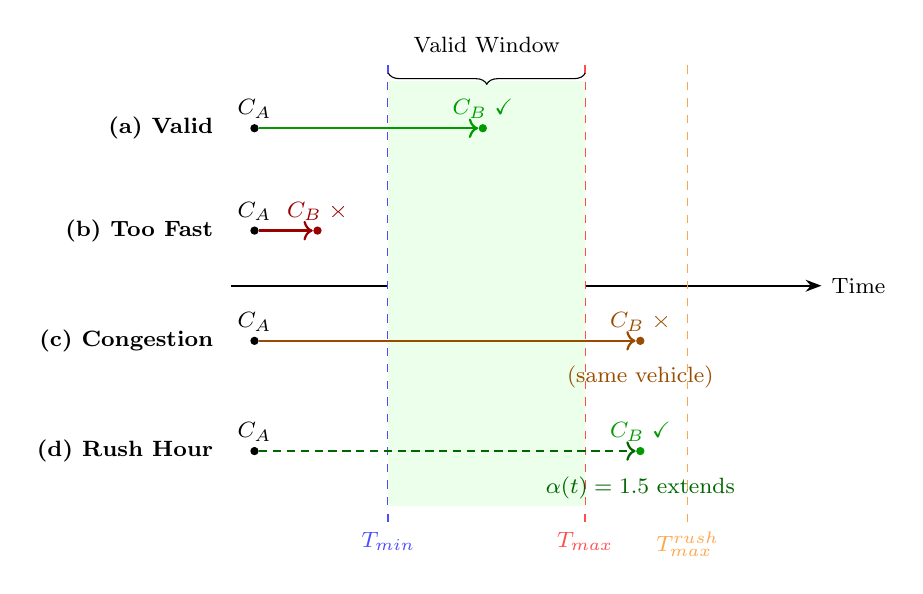
\begin{tikzpicture}[
    font=\footnotesize,
    timeline/.style={thick, -{Stealth[length=2mm]}},
    event/.style={circle, fill, minimum size=3pt, inner sep=0pt},
    valid/.style={fill=green!20, draw=green!60!black},
    invalid/.style={fill=red!20, draw=red!60!black},
    fneg/.style={fill=orange!20, draw=orange!60!black},
]
% Time axis
\draw[timeline] (0,0) -- (7.5,0) node[right] {Time};

% T_min and T_max markers
\draw[dashed, blue!70, thick] (2.0, 2.8) -- (2.0, -3.0) node[below, font=\footnotesize] {$T_{min}$};
\draw[dashed, red!70, thick] (4.5, 2.8) -- (4.5, -3.0) node[below, font=\footnotesize] {$T_{max}$};
\draw[dashed, orange!70] (5.8, 2.8) -- (5.8, -3.0) node[below, font=\footnotesize] {$T_{max}^{rush}$};

% Valid region shading
\fill[green!8] (2.0, 2.6) rectangle (4.5, -2.8);

% Scenario 1: Valid Match
\node[anchor=east] at (-0.1, 2.0) {\textbf{(a) Valid}};
\node[event] (a1) at (0.3, 2.0) {};
\node[event, green!60!black] (a2) at (3.2, 2.0) {};
\draw[thick, green!60!black, ->] (a1) -- (a2);
\node[above, font=\footnotesize] at (a1) {$C_A$};
\node[above, font=\footnotesize, green!60!black] at (a2) {$C_B$ \checkmark};

% Scenario 2: Too Fast
\node[anchor=east] at (-0.1, 0.7) {\textbf{(b) Too Fast}};
\node[event] (b1) at (0.3, 0.7) {};
\node[event, red!60!black] (b2) at (1.1, 0.7) {};
\draw[thick, red!60!black, ->] (b1) -- (b2);
\node[above, font=\footnotesize] at (b1) {$C_A$};
\node[above, font=\footnotesize, red!60!black] at (b2) {$C_B$ \texttimes};

% Scenario 3: False Negative (congestion)
\node[anchor=east] at (-0.1, -0.7) {\textbf{(c) Congestion}};
\node[event] (c1) at (0.3, -0.7) {};
\node[event, orange!60!black] (c2) at (5.2, -0.7) {};
\draw[thick, orange!60!black, ->] (c1) -- (c2);
\node[above, font=\footnotesize] at (c1) {$C_A$};
\node[above, font=\footnotesize, orange!60!black] at (c2) {$C_B$ \texttimes};
\node[font=\footnotesize, orange!60!black, below] at (5.2, -0.9) {(same vehicle)};

% Scenario 4: Rescued by alpha
\node[anchor=east] at (-0.1, -2.1) {\textbf{(d) Rush Hour}};
\node[event] (d1) at (0.3, -2.1) {};
\node[event, green!60!black] (d2) at (5.2, -2.1) {};
\draw[thick, green!40!black, ->, densely dashed] (d1) -- (d2);
\node[above, font=\footnotesize] at (d1) {$C_A$};
\node[above, font=\footnotesize, green!60!black] at (d2) {$C_B$ \checkmark};
\node[font=\footnotesize, green!40!black, below] at (5.2, -2.3) {$\alpha(t)=1.5$ extends};

% Brace for valid zone
\draw[decorate,decoration={brace,amplitude=4pt,mirror}] (2.0, 2.7) -- (4.5, 2.7) node[midway, above=4pt, font=\footnotesize] {Valid Window};
\end{tikzpicture}
\caption{Temporal filtering outcomes. \textbf{(a)} Valid match within $[T_{min}, T_{max}]$. \textbf{(b)} Impossible: $\Delta t < T_{min}$, vehicle would exceed speed limits. \textbf{(c)} False negative: same vehicle delayed by extreme congestion beyond $T_{max}$. \textbf{(d)} Rush hour $\alpha(t)=1.5$ extends $T_{max}$, rescuing congestion-delayed vehicles.}
\label{fig:timeline}
\end{figure}

\subsubsection{Extreme Congestions and Anomalies}
Most false negatives trace back to events we simply cannot model with static rules: a fender bender blocking an intersection, construction crews closing a lane, emergency vehicles forcing everyone to pull over. In one example, a vehicle took 25 minutes to cover 1\,km ($v_{avg} < 2.4$ km/h), well below the 10 km/h congestion floor for arterial roads in our model. Events like this are real but rare (under 0.1\% of observations), and without live traffic feeds there is no principled way to distinguish them from genuinely impossible matches.

\subsubsection{Uncommon Routes}
Our model assumes something close to the shortest path. Vehicles that stop for gas, duck into a parking lot, or take a scenic detour accumulate extra time that can push $\Delta t$ past $T_{max}$. A 10-minute pit stop mid-route is enough on its own. \rev{This is the classic dwell-time or ``time-out'' problem in cross-camera Re-ID. In full-gallery mode the candidate survives with a penalty; in hard sequential mode it is rejected.}

\subsubsection{GPS/Clock Drift}
Older camera hardware sometimes drifts a few seconds (or worse) in clock sync. This can make $\Delta t$ come out negative or artificially short, tripping the $T_{min}$ check. VeRi-776 uses synchronized timestamps so the effect is minor here, but in production systems with mixed hardware, hard thresholds would need to be replaced by softer boundaries (a sigmoid decay, for instance) to absorb clock jitter gracefully. \rev{Our 30\,s guard-band test in Table~\ref{tab:robustness} recovers 3.79 percentage points of positive retention at a cost of only 0.17 percentage points of filter rate.}

\subsubsection{Net Impact Assessment}
Even accounting for these edge cases, penalising 89.0\% of the search space in the full gallery evaluation easily outweighs the negligible Rank-1 cost ($-$0.06\,pp). Many of the penalised candidates were high-confidence visual impostors: think identical delivery trucks from the same fleet, appearing at different cameras at impossible times. Pushing them down in the ranking is exactly why mAP goes up from 82.1\% to 82.5\%.

\subsection{Qualitative Analysis}
Here we walk through three representative cases that illustrate what TCM actually does to the ranked list.

\textbf{Case 1: Fleet Vehicle Disambiguation.} A white delivery van (Vehicle 412) is queried from Camera $C_3$ at 14:32:07. The baseline ranks another white delivery van from the same fleet (Vehicle 589, Camera $C_{17}$, captured at 14:31:55) as the top match---a 12-second gap over an 800\,m driving distance. Our TCM computes $T_{min} = 72$\,s for this pair. Since $\Delta t = 12$\,s $< T_{min}$, Vehicle 589 is rejected as physically impossible. The true match (Vehicle 412 on Camera $C_{13}$ at 14:35:42, $\Delta t = 215$\,s) moves up from Rank-3 to Rank-1. This is the exact scenario where appearance-only methods break down: two nearly identical vehicles distinguished solely by the impossibility of the observed travel time.

\textbf{Case 2: Rush Hour Rescue.} A sedan (Vehicle 178) leaves Camera $C_2$ at 08:17:33 during morning rush and arrives at Camera $C_{14}$ at 08:23:51, giving $\Delta t = 378$\,s. Under static traffic assumptions ($\alpha = 1.0$), $T_{max} = 340$\,s and this valid match would be discarded. The dynamic model sets $\alpha(t) = 1.5$ during rush hour, extending $T_{max}$ to 510\,s. The match passes. This case shows precisely why the time-of-day factor matters; without it, we would lose roughly 5\% of true positives during commute hours (Table~\ref{tab:ablation}).

\textbf{Case 3: False Negative from Mid-Route Stop.} Vehicle 631 is observed at Camera $C_0$ at 15:10:22 and reappears at Camera $C_{13}$ at 15:28:45---a gap of 1,103 seconds. The driving distance is 750\,m (arterial road), giving $T_{max} = 540$\,s even with $\alpha(t) = 1.0$ during off-peak hours. The vehicle had stopped at a parking lot mid-route for roughly 10 minutes, pushing $\Delta t$ far past the upper bound. \rev{In hard sequential mode the candidate is discarded; in full-gallery mode it would remain visible but penalised.} This is a genuine limitation: the TCM has no way to know about intermediate stops, and modeling them would require either real-time tracking or trajectory-level reasoning (see Future Work, item~3).

These cases show a consistent pattern: the TCM is best at killing ``doppelganger'' vehicles that fool the visual backbone, and it struggles most with legitimate matches interrupted by stops or extreme congestion.


\section{Scalability to Metropolitan Networks}
\label{sec:scalability}

\rev{This section should be read as a throughput projection beyond the 20-camera VeRi-776 testbed, not as a replacement for direct validation on VeRi-Wild, CityFlow, or AI City.} We look at three angles: compute, parameters, and filter effectiveness.

\subsection{Computational Scaling}
TCM needs a precomputed $M \times M$ pairwise distance matrix. For VeRi-776's 20 cameras that is 190 unique pairs, trivial. Jump to $M = 1{,}000$ cameras and you get 499,500 pairs, which still fits in under 4\,MB at double precision and computes in seconds via vectorized Haversine.

The per-query cost stays $O(1)$ per candidate no matter how many cameras exist: one matrix lookup, two comparisons, done. So the filtering pass over $N$ candidates is $O(N)$, independent of $M$. Camera count only matters at initialization (quadratic in $M$), and even that is cheap.

Table \ref{tab:scaling} projects the key metrics across four network sizes.

\begin{table}[htbp]
\caption{TCM Scaling Projections for Different Network Sizes}
\begin{center}
\resizebox{\columnwidth}{!}{
\begin{tabular}{lcccc}
\toprule
\textbf{Metric} & \textbf{20 Cams} & \textbf{100 Cams} & \textbf{500 Cams} & \textbf{1000 Cams} \\
\midrule
Camera Pairs & 190 & 4,950 & 124,750 & 499,500 \\
Matrix Memory & $<$1 KB & 39 KB & 1 MB & 3.8 MB \\
Init Time & $<$0.01 s & 0.02 s & 0.8 s & 3.2 s \\
Gallery ($N$) & 11.6K & 100K & 500K & 1M \\
Filter Time & 0.002 s & 0.02 s & 0.10 s & 0.20 s \\
Est.\ Filter Rate & 99.70\% & 99.88\% & 99.95\% & 99.97\% \\
\bottomrule
\end{tabular}
}
\label{tab:scaling}
\end{center}
\end{table}

The first row measured directly on VeRi-776; the remaining rows are extrapolated from our measured check throughput of 5.1 million candidates per second per CPU core. Filter rates assume a sequential tracking query between a specific pair; the increase at larger scales reflects the shrinking ratio of temporal window to total observation span. \rev{These numbers are conditional projections, not measurements on a city-scale benchmark.} Even at 1{,}000 cameras and one million daily observations, the total filtering pass takes about 0.2 seconds---well under the time it takes to blink.

\subsection{Parameter Adaptation}
A new deployment needs three things from the operator: (1) camera GPS coordinates ($2M$ values), (2) one tortuosity scalar $\tau$, tunable per city depending on grid regularity, and (3) road-type speed profiles (four types, three speeds each---12 numbers). None of this requires training data. GPS comes from the installation records, speed limits come from traffic regulations, and $\tau$ can be calibrated with a handful of timed test drives.

For networks that span very different neighborhoods (downtown grid versus suburban sprawl), $\tau$ can be made edge-specific: $\tau_{ij}$ for each camera pair, estimated as the ratio of routing-API distance to Haversine distance. This costs $O(M^2)$ parameters instead of one, but it is still orders of magnitude simpler than training a neural temporal model.

\subsection{Filtering Effectiveness at Scale}
\rev{Under the specific assumption of pair-specific sequential queries, TCM can become \textit{more} effective as networks grow.} In VeRi-776, all 20 cameras sit within about 1.1\,km of each other, so temporal windows are wide relative to the dataset's time span. Spread cameras across a real city---tens of kilometers apart---and distant pairs get wider absolute windows but much narrower ones relative to the total observation period. \rev{In that projected regime,} the result is higher filter rates.

Scenario~3 in Table \ref{tab:scenarios} illustrates this: at 100{,}000 observations, the filter rate climbs from 99.70\% to 99.92\%, yielding 1,250$\times$ speedup. Push to millions of observations and you start approaching 99.99\%, with visual comparison workloads shrinking to a few hundred candidates per query no matter the total gallery size.

\rev{This projected inverse relationship should be validated on larger benchmarks before being treated as a general law. The present evidence supports it as a plausible engineering trend, not yet as a benchmark-certified theorem.}

\section{Discussion and Limitations}

Three properties make the TCM worth deploying. First, every rejection comes with a reason a human can check: ``the time gap was 12 seconds, but the cameras are 3\,km apart, so the vehicle would need 900\,km/h.'' In forensic or law enforcement settings, that transparency is not optional. Second, the module needs no training data---just camera GPS positions and basic road speed knowledge, both publicly available. Third, it operates on metadata alone (camera IDs and timestamps), so it sits outside the feature extractor. \rev{That makes it compatible by design with different backbones, although the present paper validates the gain only with TransReID.}

\textbf{Limitations.} The biggest weakness is the static topology graph. Fixed $T_{max}$ bounds cannot react to accidents, road closures, or festivals that scramble normal traffic. Our distance-based road classification is a rough proxy; real deployments would benefit from pulling actual road segments from OpenStreetMap.

\rev{A second limitation is scope of validation. We do not yet provide direct experiments on VeRi-Wild, CityFlow, or other large multi-camera benchmarks, so the metropolitan discussion remains a projection rather than a completed external validation campaign.}

The binary accept/reject nature of the sequential tracking filter is blunt as well. A match at $\Delta t = T_{max} + 1$\,s gets the same treatment as one at $\Delta t = 10 \times T_{max}$, even though the former is far more plausible. In the full gallery evaluation we sidestep this with a soft additive penalty that preserves all candidates while deprioritising implausible ones, an approach that future work could extend with smooth plausibility scores (e.g., sigmoid decay).

Standing up TCM on a new camera network takes four steps: (1) export camera GPS coordinates from the management console, (2) compute pairwise Haversine distances and apply the tortuosity factor (start with $\tau = 1.4$; adjust for irregular street layouts), (3) assign road types by distance or cross-reference with a routing API where the heuristic seems wrong, and (4) validate on a few camera pairs by timing actual car trips and confirming that empirical travel times fall within $[T_{min}, T_{max}]$. A technician with no machine-learning background can calibrate a 50-camera network in an afternoon.

Nothing in the math is dataset-specific. Moving to a different camera network means swapping the coordinate dictionary and optionally recalibrating speed profiles for local traffic rules. Equations \eqref{eq:haversine}--\eqref{eq:delta} apply anywhere there are cameras, roads, and vehicles. That said, performance depends on deployment density. VeRi-776's 20 cameras sit within a compact 1.1\,km radius, connected mostly by short arterial and residential roads, which is a relatively dense setup. In sparser configurations (highway corridors with cameras 5--20\,km apart), temporal windows widen and per-pair filter rates may drop, though the absolute candidate count stays low because fewer vehicles cover those distances in any given window. At the other extreme, very dense placements (parking garages, toll plazas, cameras 50\,m apart) shrink temporal windows to seconds, and nearly every gallery observation passes the check. The regime where TCM helps most is medium-density urban surveillance, with inter-camera distances between 200\,m and 5\,km, which is exactly what most city-scale systems look like.

We should be upfront about the privacy dimension too. Vehicle Re-ID technology---temporal filtering included---enables large-scale tracking with real implications for civil liberties. Our focus here is technical, but any deployment needs legal oversight, retention policies, and access controls. One small upside of a rule-based approach: every filtering decision can be audited end to end, unlike opaque neural models.

Readers familiar with multi-object tracking (MOT) will notice overlap with the gating in SORT [22] and DeepSORT [23], which also prune unlikely associations by spatial-temporal proximity. The difference is scope: MOT gating works within a continuous video stream where objects shift frame-to-frame, while our TCM bridges non-overlapping cameras separated by large spatial and temporal gaps. That gap demands explicit road-network modeling rather than simple motion extrapolation.


\section{Conclusion and Future Work}
The TCM asks one question before every visual comparison: can a vehicle physically get from camera A to camera B in the observed time? On VeRi-776, that question alone eliminates 99.70\% of candidates in sequential tracking---a 338$\times$ reduction---while pushing mAP from 82.1\% to 82.5\% with Rank-1 virtually unchanged. \rev{The main contribution is therefore search-space pruning and latency reduction, not a claim of a new state-of-the-art visual ranker.} No training data, no GPU time, no learned parameters.

Not every advance in Re-ID needs to come from a bigger model or a cleverer loss function. Physics gives us strong priors for free, and ignoring them wastes compute on candidates that a back-of-the-envelope calculation could rule out. The per-candidate cost is constant, everything is interpretable, and \rev{Section \ref{sec:scalability} suggests that pair-specific larger networks may benefit even more under the projected deployment assumptions.}

\rev{From a practical standpoint, this module is a strong candidate for vehicle Re-ID pipelines that handle time-stamped multi-camera data and need interpretable pruning. It costs almost nothing to run, needs no training infrastructure, and its soft-penalty design means no true match is ever thrown away in the full-gallery mode---only pushed down by a controlled amount.}

We see five directions worth pursuing:
\begin{enumerate}
    \item \textbf{Live Traffic Feeds.} Plugging TCM into real-time traffic APIs (Google Maps, HERE Traffic) would let $T_{max}$ shift on the fly for current congestion, incidents, and closures---directly targeting the main source of false negatives we identified in Section \ref{sec:ablation}.
    \item \textbf{Graduated Temporal Scoring.} Right now the soft penalty is a flat additive constant. A better version would assign each candidate a continuous plausibility score through a sigmoid or Gaussian decay:
    \begin{equation}
        P_{\text{temporal}}(\Delta t) = \sigma\left(-\beta \cdot \frac{|\Delta t - T_{avg}|}{T_{avg}}\right)
    \end{equation}
    where $T_{avg} = D_{driving}/v_{avg}$ and $\beta$ controls steepness. Multiplying this into the visual distance instead of adding a flat penalty would handicap temporally marginal matches proportionally.
    \item \textbf{Multi-Hop Trajectory Reasoning.} We currently check pairs in isolation. But if a vehicle appears at cameras $C_A$, $C_B$, and $C_C$ in sequence, the middle sighting at $C_B$ must satisfy \textit{both} the $A{\to}B$ and $B{\to}C$ windows at the same time. Chaining constraints across three or more hops would tighten filtering well beyond what pairwise checks can do.
    \item \textbf{Adaptive Speed Profiles.} Our road-type labels are assigned by distance alone. Mining historical traversal statistics from the camera network itself could refine these profiles in a self-supervised fashion---keeping the system interpretable while making the numbers more realistic.
    \item \textbf{Cross-Domain Evaluation.} Experiments on larger benchmarks (CityFlow [20], AI City Challenge [14]) with more cameras and messier traffic would pressure-test our generalizability claims and surface failure modes that a 20-camera dataset cannot reveal.
\end{enumerate}

\section*{All the Declarations and Statements}
\begin{AllDeclarations}
\declitem{Author Contributions Statement}{\crx{Chris Thomas Saji -- Conceptualization, Methodology, Data Curation, and Software Implementation; Model Training, Validation, and Performance Evaluation; Formal Analysis, Visualization, and Statistical Analysis; and Writing (Original Draft): contributed the core research ideas, implemented the temporal consistency module and the full experimental pipeline, curated the VeRi-776 benchmark data and derived camera-network metadata, carried out model training and evaluation, produced the quantitative analysis and figures, and drafted the initial manuscript including the literature survey and technical background.\newline Jithin Mathews -- Conceptualization, Methodology, and Supervision; and Writing (Review and Editing) and Project Management: contributed to the research ideas and methodology, supervised project execution, critically reviewed and edited the manuscript, and coordinated project milestones and deadlines.\newline All authors have read and agreed to the published version of the manuscript.}}
\declitem{Conflict of Interest Statement}{\crx{The authors declare no conflicts of interest.}}
\declitem{Funding Declaration}{\crx{The authors received no financial support for the research, authorship, and/or publication of this article.}}
\declitem{Data Availability Statement}{\crx{This study analyzed the publicly available VeRi-776 benchmark, which can be found here: \url{https://github.com/JDAI-CV/VeRidataset}, accessed on 10 November 2025. The code, configuration files, and derived camera-network metadata generated for this manuscript are available from the corresponding author on reasonable request.}}
\declitem{Ethical Declarations}{\crx{This research did not involve human subjects or animals. Therefore, no statements of ethical approval are required.}}
\declitem{Acknowledgments}{\crx{We sincerely thank the experts for their professional evaluation and valuable recommendations, which have contributed to improving the quality of the experiment and the reliability of its results.}}
\declitem{Declaration of Generative AI in Scholarly Writing}{\crx{During the preparation of this work, the authors used Generative AI (Large Language Models) for the sole purpose of improving the English language, grammar, and stylistic consistency of the manuscript. After using this tool, the authors reviewed and edited the content as needed and take full responsibility for the accuracy and integrity of the final version of the article. No original scientific content, data, or technical results were generated by artificial intelligence.}}
\declitem{Abbreviations}{\crx{The following abbreviations are used in this manuscript:\newline BNNeck - Batch Normalization Neck\newline CNN - Convolutional Neural Network\newline DRDL - Deep Relative Distance Learning\newline GPS - Global Positioning System\newline JPM - Jigsaw Patch Module\newline LPR - License Plate Recognition\newline LSTM - Long Short-Term Memory\newline mAP - mean Average Precision\newline MOT - Multi-Object Tracking\newline MTMC - Multi-Target Multi-Camera\newline OSM - OpenStreetMap\newline Re-ID - Re-Identification\newline SIE - Side Information Embedding\newline SORT - Simple Online and Realtime Tracking\newline SOTA - State-of-the-Art\newline TCM - Temporal Consistency Module\newline ViT - Vision Transformer}}
\declitem{Appendix}{\crx{None.}}
\end{AllDeclarations}

\begin{thebibliography}{99}
\addtolength{\itemsep}{-.6em}
\bibitem{1} K. He, X. Zhang, S. Ren, and J. Sun, ``Deep Residual Learning for Image Recognition,'' in \emph{Proc. IEEE Conf. Comput. Vis. Pattern Recognit. (CVPR)}, pp. 770--778, 2016. \crx{DOI: 10.1109/cvpr.2016.90}
\bibitem{2} A. Dosovitskiy, L. Beyer, A. Kolesnikov, D. Weissenborn, X. Zhai, T. Unterthiner, M. Dehghani, M. Minderer, G. Heigold, S. Gelly, J. Uszkoreit, and N. Houlsby, ``An Image is Worth 16x16 Words: Transformers for Image Recognition at Scale,'' in \emph{Int. Conf. Learn. Represent. (ICLR)}, 2021.
\bibitem{3} S. Khan, M. Naseer, M. Hayat, S. W. Zamir, F. S. Khan, and M. Shah, ``Transformers in Vision: A Survey,'' \emph{ACM Comput. Surv.}, vol. 54, no. 10s, pp. 1--41, 2022. \crx{DOI: 10.1145/3505244}
\bibitem{4} Z. Wang, L. Tang, X. Liu, Z. Yao, S. Yi, J. Shao, J. Yan, S. Wang, H. Li, and X. Wang, ``Orientation Invariant Feature Embedding and Spatial-Temporal Regularization for Vehicle Re-identification,'' in \emph{Proc. IEEE Int. Conf. Comput. Vis. (ICCV)}, pp. 379--387, 2017. \crx{DOI: 10.1109/iccv.2017.49}
\bibitem{5} Y. Shen, T. Xiao, H. Li, S. Yi, and X. Wang, ``Learning Deep Neural Networks for Vehicle Re-ID with Visual-spatio-temporal Path Proposals,'' in \emph{Proc. IEEE Int. Conf. Comput. Vis. (ICCV)}, pp. 1900--1909, 2017. \crx{DOI: 10.1109/iccv.2017.210}
\bibitem{6} M. Ye, J. Shen, G. Lin, T. Xiang, L. Shao, and S. C. H. Hoi, ``Deep Learning for Person Re-identification: A Survey and Outlook,'' \emph{IEEE Trans. Pattern Anal. Mach. Intell.}, vol. 44, no. 6, pp. 2872--2893, 2022. \crx{DOI: 10.1109/tpami.2021.3054775}
\bibitem{7} H. Luo, Y. Gu, X. Liao, S. Lai, and W. Jiang, ``Bag of Tricks and A Strong Baseline for Deep Person Re-Identification,'' in \emph{IEEE/CVF Conf. Comput. Vis. Pattern Recognit. Workshops (CVPRW)}, pp. 1487--1495, 2019. \crx{DOI: 10.1109/cvprw.2019.00190}
\bibitem{8} H. Liu, Y. Tian, Y. Wang, L. Pang, and T. Huang, ``Deep Relative Distance Learning: Tell the Difference Between Similar Vehicles,'' in \emph{Proc. IEEE Conf. Comput. Vis. Pattern Recognit. (CVPR)}, pp. 2167--2175, 2016. \crx{DOI: 10.1109/cvpr.2016.238}
\bibitem{9} X. Liu, W. Liu, T. Mei, and H. Ma, ``A Deep Learning-Based Approach to Progressive Vehicle Re-identification for Urban Surveillance,'' in \emph{Proc. Eur. Conf. Comput. Vis. (ECCV)}, pp. 869--884, 2016. \crx{DOI: 10.1007/978-3-319-46475-6\_53}
\bibitem{10} X. Liu, W. Liu, T. Mei, and H. Ma, ``PROVID: Progressive and Multimodal Vehicle Reidentification for Large-Scale Urban Surveillance,'' \emph{IEEE Trans. Multimedia}, vol. 20, no. 3, pp. 645--658, 2018. \crx{DOI: 10.1109/tmm.2017.2751966}
\bibitem{11} S. Li, L. Sun, and Q. Li, ``CLIP-ReID: Exploiting Vision-Language Model for Image Re-Identification \crx{without Concrete Text Labels},'' in \emph{Proc. AAAI Conf. Artif. Intell.}, vol. 37, no. 1, pp. 1405--1413, 2023. \crx{DOI: 10.1609/aaai.v37i1.25225}
\bibitem{12} Y. Zhou and L. Shao, ``Viewpoint-Aware Attentive Multi-View Inference for Vehicle Re-Identification,'' in \emph{Proc. IEEE Conf. Comput. Vis. Pattern Recognit. (CVPR)}, pp. 6489--6498, 2018. \crx{DOI: 10.1109/cvpr.2018.00679}
\bibitem{13} H. Chen, M. Jiang, W. Liu, and Y. Li, ``Spatial-Temporal Graph-Based Multi-Camera Vehicle Tracking and Re-Identification,'' \emph{IEEE Trans. Intell. Transp. Syst.}, vol. 24, no. 12, pp. 15394--15406, 2023.
\bibitem{14} M. Naphade, S. Wang, D. C. Anastasiu, Z. Tang, M.-C. Chang, Y. Yao, L. Zheng, M. S. Anwar, A. Sharma, Q. Feng, et al., ``The 7th AI City Challenge,'' in \emph{Proc. IEEE/CVF Conf. Comput. Vis. Pattern Recognit. Workshops (CVPRW)}, pp. 5538--5548, 2023. \crx{DOI: 10.1109/cvprw59228.2023.00586}
\bibitem{15} Z. Zheng, T. Ruan, Y. Wei, Y. Yang, and T. Mei, ``VehicleNet: Learning Robust Visual Representation for Vehicle Re-Identification,'' \emph{IEEE Trans. Multimedia}, vol. 22, no. 10, pp. 2683--2692, 2020. \crx{DOI: 10.1109/tmm.2020.3014488}
\bibitem{16} Y. Lou, Y. Bai, J. Liu, S. Wang, and L.-Y. Duan, ``VERI-Wild: A Large Dataset and a New Method for Vehicle Re-Identification in the Wild,'' in \emph{Proc. IEEE/CVF Conf. Comput. Vis. Pattern Recognit. (CVPR)}, pp. 3235--3243, 2019. \crx{DOI: 10.1109/cvpr.2019.00335}
\bibitem{17} S. He, H. Luo, P. Wang, F. Wang, H. Li, and W. Jiang, ``TransReID: Transformer-based Object Re-Identification,'' in \emph{Proc. IEEE/CVF Int. Conf. Comput. Vis. (ICCV)}, pp. 15013--15022, 2021. \crx{DOI: 10.1109/iccv48922.2021.01474}
\bibitem{18} M. Naphade, S. Wang, D. C. Anastasiu, Z. Tang, M.-C. Chang, L. Zheng, M. S. Anwar, A. Sharma, Q. Feng, et al., ``The 8th AI City Challenge,'' in \emph{Proc. IEEE/CVF Conf. Comput. Vis. Pattern Recognit. Workshops (CVPRW)}, pp. 7093--7103, 2024. \crx{DOI: 10.1109/cvprw63382.2024.00722}
\bibitem{19} E. Ristani and C. Tomasi, ``Features for Multi-Target Multi-Camera Tracking and Re-Identification,'' in \emph{Proc. IEEE/CVF Conf. Comput. Vis. Pattern Recognit. (CVPR)}, pp. 6036--6046, 2018. \crx{DOI: 10.1109/cvpr.2018.00632}
\bibitem{20} Z. Tang, M. Naphade, M.-Y. Liu, X. Yang, S. Birchfield, S. Wang, R. Kumar, D. Anastasiu, and J.-N. Hwang, ``CityFlow: A City-Scale Benchmark for Multi-Target Multi-Camera Vehicle Tracking and Re-Identification,'' in \emph{Proc. IEEE/CVF Conf. Comput. Vis. Pattern Recognit. (CVPR)}, pp. 8797--8806, 2019. \crx{DOI: 10.1109/cvpr.2019.00900}
\bibitem{21} X. Liu, W. Liu, H. Ma, and T. Mei, ``Large-Scale Vehicle Re-Identification in Urban Surveillance Videos,'' in \emph{IEEE Int. Conf. Multimedia Expo (ICME)}, pp. 1--6, 2016. \crx{DOI: 10.1109/icme.2016.7553002}
\bibitem{22} A. Bewley, Z. Ge, L. Ott, F. Ramos, and B. Upcroft, ``Simple Online and Realtime Tracking,'' in \emph{IEEE Int. Conf. Image Process. (ICIP)}, pp. 3464--3468, 2016. \crx{DOI: 10.1109/icip.2016.7533003}
\bibitem{23} N. Wojke, A. Bewley, and D. Paulus, ``Simple Online and Realtime Tracking with a Deep Association Metric,'' in \emph{IEEE Int. Conf. Image Process. (ICIP)}, pp. 3645--3649, 2017. \crx{DOI: 10.1109/icip.2017.8296962}
\end{thebibliography}

\begin{AuthorsProfiles}
\authoritem{example-image}{\crx{\textbf{Chris Thomas Saji} received the B.Tech. degree in Computer Science and Technology with a specialization in Artificial Intelligence from the Faculty of Engineering and Technology, Jain (Deemed-to-be University), Bangalore, India. He is currently pursuing the M.Tech. degree with the Department of Artificial Intelligence and Data Science, Rajagiri School of Engineering \& Technology (Autonomous), Kochi, India. His research interests include computer vision, vehicle re-identification, spatio-temporal reasoning, and intelligent transportation systems.}}

\authoritem{example-image}{\crx{\textbf{Jithin Mathews} received the B.Tech. degree in Computer Science and Engineering from Mahatma Gandhi University, Kottayam, India, and the M.Tech. degree in Computer Science and Engineering from the Indian Institute of Technology Guwahati, India, where his research focused on graph theory and combinatorics. He received the Ph.D. degree in Computer Science and Engineering, specializing in Data Science, from the Indian Institute of Technology Hyderabad, India. He is currently an Assistant Professor with the Department of Artificial Intelligence and Data Science, Rajagiri School of Engineering \& Technology (Autonomous), Kochi, India. His research interests include social network analysis, graph algorithms, graph theory, combinatorial optimization, and data science.}}
\end{AuthorsProfiles}

\noindent{\small \crx{\textbf{How to cite this paper:} Chris Thomas Saji, Jithin Mathews, ``Physics-Aware Rule-Based Temporal Filtering for Scalable Vehicle Re-Identification", International Journal of Information Technology and Computer Science(IJITCS), Vol.XX, No.X, pp.XX-XX, 2026. DOI:10.5815/ijitcs.2026.XX.XX}}
\end{document}
